
\newpage
%%%%%%%%%%%%%%%%%%%%%%%%%%%%%%%%%%%%%%%%%%%%%%%%%%%%%%%%%%%%%%%%%%%%%%%%%%%%%%%
%%%
%%%                     FIND THE DOMAIN AND ASYMPTOTES
%%%
%%%%%%%%%%%%%%%%%%%%%%%%%%%%%%%%%%%%%%%%%%%%%%%%%%%%%%%%%%%%%%%%%%%%%%%%%%%%%%%
\subsection*{Identify The Domain and Any Vertical Asymptote(s)}
\chead{Domain and Asymptotes}

\begin{tcolorbox}[title=Hint, colback=teal!10!white, colframe=teal!75!black]
The argument of the logarithm should be strictly positive: $\log_b\Box\Rightarrow\Box>0$
\end{tcolorbox}
\newpage
\begin{enumerate}[resume]


\item $y=\log_2(x-3)$
    {\color{blue}
    \[
    x-3>0\Rightarrow x>3
    \]

\begin{figure}[!h]
    \centering
    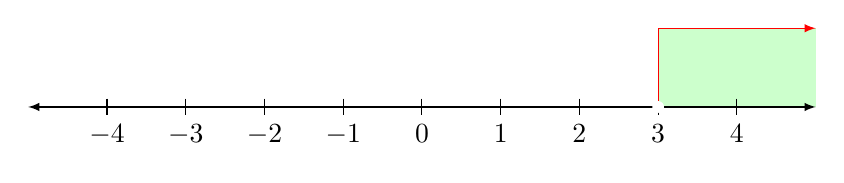
\begin{tikzpicture}
        \fill[green!20](5,0)rectangle(3,1);
        \draw[latex-latex] (-5,0) -- (5,0) ;
        \foreach \x in {-4,-3,-2,-1,0,1,2,3,4} \draw[shift={(\x,0)},color=black] (0pt,3pt) -- (0pt,-3pt) node[below] {$\x$};
        %\node[circle,fill=white,inner sep=1.5pt](a)at(0,0){};
        \node[circle,fill=white,inner sep=1.5pt](b)at(3,0){};
        %\node[circle,fill=black,inner sep=1.5pt](c)at(-3,0){};
        \draw[-latex,red](b)--++(0,1)--++(2,0);
    \end{tikzpicture}
    \caption{\color{blue}{Graphical representation of the domain of $\log_2(x-3)$}}
    \end{figure}
    
\vspace{1in}

    
    \begin{figure}[htbp]
        \centering
        \includegraphics[width=0.6\textwidth]{log1_10}
        \caption{\color{blue}{Graph of the function $\log_2(x-3)$ showing the asymptote $x=3$ and the domain $x>3$}}
        %\label{fig:myimage}
    \end{figure}
}
\begin{tcolorbox}[title=Answer, colback=blue!10!white, colframe=blue!75!black]
Domain in Interval Notation: $x\in (3,\infty)$\\
Domain in Set-builder notation: $\{ x \in \mathbb{R} \mid x>3 \}$\\
Asymptote: $x=3$
\end{tcolorbox}

\newpage    
\item $y=\ln(x^2-16)$

{\color{blue}
The argument of the lo is $x^2-16$. 
\begin{itemize}
    \item Factor the argument
    \item Find the zeros of the argument
    \item Identify the regions where each factor is positive/negative
    \item Identify the regions where the argument is positive/negative
\end{itemize}

 Factor the argument then find the zeros:
    \begin{align*}
        x^2-16&=0\\
        (x-4)(x+4)&=0\\
        x-4=0,\quad& x+4=0\\
        x=4,\quad& x=-4
    \end{align*}

    Setup a table showing the sign of each factor then the overall sign of the argument.
    \begin{align*}
        x-4>0&\Rightarrow x>4\\
        x+4>0&\Rightarrow x>-4
    \end{align*}

From the table we see that the argument is positive to the right of $x=4$ and to the left of $x=-4$. We can also see the asymptotes at $x=\pm 4$
\vspace{1in}

 \begin{figure}[!h]
    \centering    
\begin{tikzpicture}
\tkzTabInit[lgt=4,espcl=2,deltacl=0]
  { /.8, $x-4$ /.8, $x+4$ /.8, $(x-4)(x+4)$ /.8}
  {,$-4$,$4$,} % four main references
\tkzTabLine {,-,t,-,z,+,} % seven denotations
\tkzTabLine {,-,z,+,t,+,}
\tkzTabLine {,+,z,-,z,+,}
\end{tikzpicture}
\caption{}
\end{figure}

 
\newpage
\begin{figure}[!h]
    \centering
    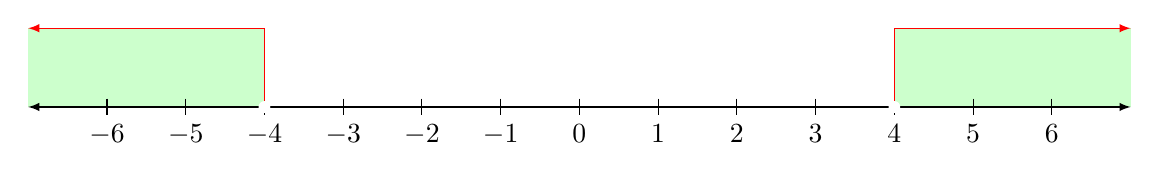
\begin{tikzpicture}
        \fill[green!20](7,0)rectangle(4,1);
        \fill[green!20](-7,0)rectangle(-4,1);
        \draw[latex-latex] (-7,0) -- (7,0) ;
        \foreach \x in {-6,-5,-4,-3,-2,-1,0,1,2,3,4,5,6} \draw[shift={(\x,0)},color=black] (0pt,3pt) -- (0pt,-3pt) node[below] {$\x$};
        \node[circle,fill=white,inner sep=1.5pt](a)at(-4,0){};
        \node[circle,fill=white,inner sep=1.5pt](b)at(4,0){};
        %\node[circle,fill=black,inner sep=1.5pt](c)at(-3,0){};
        \draw[-latex,red](a)--++(0,1)--++(-3,0);
        \draw[-latex,red](b)--++(0,1)--++(3,0);
    \end{tikzpicture}
    \caption{\color{blue}{Graphical representation of the domain of $\ln(x^2-4)$}}
    \end{figure}

\vspace{1in}
We can also identify the domain and asymptotes by plotting the function as showin below.  

    \begin{figure}[htbp]
        \centering
        \includegraphics[width=0.6\textwidth]{log1_11}
        \caption{\color{blue}{Graph of the function $\ln(x^2-16)$ showing the asymptotes $x=\pm 4$ and the domain $x\in (-\infty,-4)\cup (4,\infty)$}}
        %\label{fig:myimage}
    \end{figure}
 }   

\begin{tcolorbox}[title=Answer, colback=blue!10!white, colframe=blue!75!black]
Domain in Interval Notation: $x\in (-\infty,-4)\cup (4,\infty)$\\
Domain in Set-builder notation: $\{ x \in \mathbb{R} \mid x\ne \pm4 \}$\\
Asymptotes: $x=\pm 4$  
\end{tcolorbox}
 
\newpage
\item $y=\log(x^2+5x+6)$
    {\color{blue}
    \begin{align*}
        x^2+5x+6&=0\\
        (x+2)(x+3)&=0\\
        x+2=0,\quad&x+3=0\\
        x=-2,\quad& x=-3
    \end{align*}


    Setup a table showing the sign of each factor then the overall sign of the argument looking for regions of positive sign.
    \begin{align*}
        x+2>0&\Rightarrow x>-2\\
        x+3>0&\Rightarrow x>-3
    \end{align*}

 \begin{figure}[!h]
    \centering    
\begin{tikzpicture}
\tkzTabInit[lgt=4,espcl=2,deltacl=0]
  { /.8, $x+2$ /.8, $x+3$ /.8, $(x+2)(x+3)$ /.8}
  {,$-3$,$-2$,} % four main references
\tkzTabLine {,-,t,-,z,+,} % seven denotations
\tkzTabLine {,-,z,+,t,+,}
\tkzTabLine {,+,z,-,z,+,}
\end{tikzpicture}
%\caption{}
\end{figure}

\begin{figure}[!h]
    \centering
    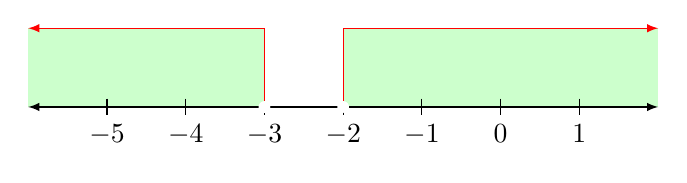
\begin{tikzpicture}
        \fill[green!20](-6,0)rectangle(-3,1);
        \fill[green!20](-2,0)rectangle(2,1);
        \draw[latex-latex] (-6,0) -- (2,0) ;
        \foreach \x in {-5,-4,-3,-2,-1,0,1} \draw[shift={(\x,0)},color=black] (0pt,3pt) -- (0pt,-3pt) node[below] {$\x$};
        \node[circle,fill=white,inner sep=1.5pt](a)at(-3,0){};
        \node[circle,fill=white,inner sep=1.5pt](b)at(-2,0){};
        %\node[circle,fill=black,inner sep=1.5pt](c)at(-3,0){};
        \draw[-latex,red](a)--++(0,1)--++(-3,0);
        \draw[-latex,red](b)--++(0,1)--++(4,0);
    \end{tikzpicture}
    \caption{\color{blue}{Graphical representation of the domain of $\log(x^2+5x+6)$}}
    \end{figure}
\newpage
    \begin{figure}[htbp]
        \centering
        \includegraphics[width=0.6\textwidth]{log1_12}
        \caption{\color{blue}{Graph of the function $\log(x^2+5x+6)$ showing the asymptotes $x=-3$ and $x=-2$ and the domain $x\in (-\infty,-3)\cup (-2,\infty)$}}
        %\label{fig:myimage}
    \end{figure}

    }

\begin{tcolorbox}[title=Domain and Asymptotes, colback=blue!10!white, colframe=blue!75!black]
Domain: Interval Notation: $x\in (-\infty,-3)\cup (-2,\infty)$\\
Domain: Set-builder notation: $\{ x \in \mathbb{R} \mid x\ne -3,-2 \}$\\
Asymptotes: $x=-3, x=-2$  
\end{tcolorbox}




\newpage
\item $y=\log\left(\sqrt{2x-1}+2\right)$
    {\color{blue}

A close look at the argument of log indicates that it cannot be zero or negative, only positive. So we just need to focus on the quantity under the square root and ensure that it's not negative.

    \begin{align*}
        2x-1&\ge 0\\
        2x&\ge 1\\
        x&\ge \frac{1}{2}
    \end{align*}

For $x\ge\frac{1}{2}$, the argument of the log is positive and real.





\begin{figure}[!h]
    \centering
    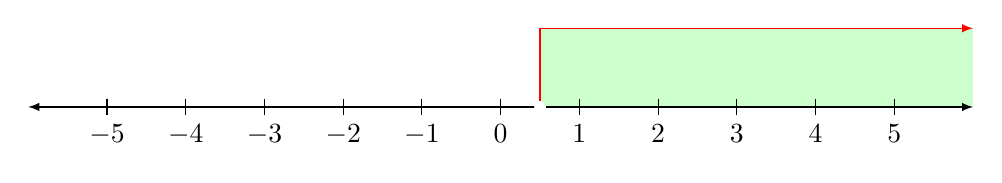
\begin{tikzpicture}
        \fill[green!20](0.5,0)rectangle(6,1);
        \draw[latex-latex] (-6,0) -- (6,0) ;
        \foreach \x in {-5,-4,-3,-2,-1,0,1,2,3,4,5} \draw[shift={(\x,0)},color=black] (0pt,3pt) -- (0pt,-3pt) node[below] {$\x$};
        \node[circle,fill=white,inner sep=1.5pt](a)at(0.5,0){};
        %\node[circle,fill=white,inner sep=1.5pt](b)at(-2,0){};
        %\node[circle,fill=black,inner sep=1.5pt](c)at(-3,0){};
        \draw[-latex,red](a)--++(0,1)--++(5.5,0);
        %\draw[-latex,red](b)--++(0,1)--++(4,0);
    \end{tikzpicture}
    \caption{\color{blue}{Graphical representation of the domain of $\log\left(\sqrt{2x-1}+2\right)$}}
    \end{figure}


    \begin{figure}[htbp]
        \centering
        \includegraphics[width=0.6\textwidth]{log1_13}
        \caption{\color{blue}{Graph of the function $\log\left(\sqrt{2x-1}+2\right)$ the domain $x\in [\frac{1}{2},\infty)$}. We can see that there we don't have an asymptote at $x=\frac{1}{2}$ - the value of the function there is finite.}
        %\label{fig:myimage}
    \end{figure}

    }
  \begin{tcolorbox}[title=Domain and Asymptotes, colback=blue!10!white, colframe=blue!75!black]
Domain: Interval Notation: $x\in [\frac{1}{2},\infty)$\\
Domain: Set-builder notation: $\{ x \in \mathbb{R} \mid x\ge \frac{1}{2}\}$\\
Asymptotes: None 
\end{tcolorbox}  
    
\newpage
\item $y=\ln\left(\dfrac{2-x}{\sqrt{x+4}}\right)$
{\color{blue}

The denominator of the argument should be real and non zero. The numerator should be strictly positive. Put these together 

    \begin{align*}
        x+4>0 &\quad\text{and}\quad 2-x>0\\
        x> -4 &\quad\text{and}\quad x < 2
    \end{align*}

Put these results in a table to get region 

 \begin{figure}[!h]
    \centering    
\begin{tikzpicture}
\tkzTabInit[lgt=4,espcl=2,deltacl=0]
  { /.8, $2-x$ /.8, $x+4$ /.8, $\frac{2-x}{\sqrt{x+4}}$ /.8}
  {,$-4$,$2$,} % four main references
\tkzTabLine {,+,t,+,z,-,} % seven denotations
\tkzTabLine {,$\nexists$,z,+,t,+,}
\tkzTabLine {,$\nexists$,t,+,t,-,}
\end{tikzpicture}
\caption{The tables shows the domain of the function is $-4<x<2$}
\end{figure}



\vspace{1in}
The domain can also be represented graphically as shown below:
\vspace{0.5in}
\begin{figure}[!h]
    \centering
    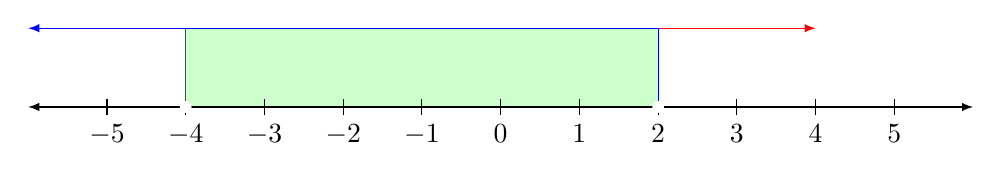
\begin{tikzpicture}
        \fill[green!20](-4,0)rectangle(2,1);

        \draw[latex-latex] (-6,0) -- (6,0) ;
        \foreach \x in {-5,-4,-3,-2,-1,0,1,2,3,4,5} \draw[shift={(\x,0)},color=black] (0pt,3pt) -- (0pt,-3pt) node[below] {$\x$};
        \node[circle,fill=white,inner sep=1.5pt](a)at(-4,0){};
        \node[circle,fill=white,inner sep=1.5pt](b)at(2,0){};
        %\node[circle,fill=black,inner sep=1.5pt](c)at(-3,0){};
        \draw[-latex,red](a)--++(0,1)--++(8,0);
        \draw[-latex,blue](b)--++(0,1)--++(-8,0);
    \end{tikzpicture}
    \caption{\color{blue}{Graphical representation of the domain of $y=\ln\left(\dfrac{2-x}{\sqrt{x+4}}\right)$}}
    \end{figure}

\newpage
    \begin{figure}[htbp]
        \centering
        \includegraphics[width=0.6\textwidth]{log1_14}
        \caption{\color{blue}{Graph of the function $y=\ln\left(\dfrac{2-x}{\sqrt{x+4}}\right)$ showing the domain $x\in (-4,2)$. We also have two asymptotes at $x=-4$ and $x=2$}}
        %\label{fig:myimage}
    \end{figure}

\vspace{1in}
\begin{tcolorbox}[title=Domain and Asymptotes, colback=blue!10!white, colframe=blue!75!black]
Domain: Interval Notation: $x\in (-4,2)$\\
Domain: Set-builder notation: $\{ x \in \mathbb{R} \mid -4<x<2\}$\\
Asymptotes: $x=-4$ and $x=2$. 
\end{tcolorbox}


    }






\newpage
\item $y=\log_2(x^2+1)-3x$
{\color{blue}

The argument of the log should be strictly positive.  But the argument $x^2+1$ is always positive (this is a parabola $x^2$ that is shifted up 1 unit so it does not touch or cross the $x-$axis). So, there are no restrictions on $x$. The second term, $-3x$,  is a monomial and its domain is $\mathbb{R}$. 

Thus the domain of the function is $\mathbb{R}$ and it has no vertical asymptotes. This can be verified from the graph below. 

\vspace{0.5in}
    \begin{figure}[htbp]
        \centering
        \includegraphics[width=0.9\textwidth]{log1_15}
        \caption{\color{blue}{Graph of the function $y=\log_2(x^2+1)-3x$ showing the domain $x\in (-\infty,\infty)$. This function does not have any asymptotes.}}
        %\label{fig:myimage}
    \end{figure}

\vspace{0.5in}
\begin{tcolorbox}[title=Domain and Asymptotes, colback=blue!10!white, colframe=blue!75!black]
Domain: Interval Notation: $x\in (-\infty,\infty)$\\
Domain: Set-builder notation: $\{ x \in \mathbb{R}\}$\\
Asymptotes: None 
\end{tcolorbox}


}



\newpage
\item $y=\log(x+3)^2$
{\color{blue}

The argument of the log, $(x+3)^2$ will never be negative (for real values of $x$) but can be zero at $x=-3$.  Thus, the domain of the function is the real numbers excluding -3, where we have a vertical asymptote.
\vspace{0.5in}
    \begin{figure}[htbp]
        \centering
        \includegraphics[width=0.6\textwidth]{log1_16}
        \caption{\color{blue}{Graph of the function $y=\log(x+3)^2$ showing the domain $x\in (-\infty,-3)\cup(-3,\infty)$. We also have an asymptote at $x=-3$}}
        %\label{fig:myimage}
    \end{figure}

\vspace{0.5in}
\begin{tcolorbox}[title=Domain and Asymptotes, colback=blue!10!white, colframe=blue!75!black]
Domain: Interval Notation: $x\in (-\infty,-3)\cup(-3,\infty)$\\
Domain: Set-builder notation: $\{ x \in \mathbb{R} \mid c\ne 3\}$\\
Asymptotes: $x=-3$ 
\end{tcolorbox}


}


\newpage
\item $y=\log\left(\dfrac{x-3}{x+2}\right)$
{\color{blue}

The domain of the function depends on the sign and values of the ratio. First find the zeros by setting each term to zero

    \begin{align*}
        x+3=0 &\quad\text{and}\quad x+2=0\\
        x= -3 &\quad\text{and}\quad x= -2
    \end{align*}

Find the regions where each factor is positive (otherwise it's negative)
    \begin{align*}
        x-3>0 &\quad\text{and}\quad x+2>0\\
        x> -3 &\quad\text{and}\quad x > -2
    \end{align*}

Setup a table to get the overall signs of the quotient:

 \begin{figure}[!h]
    \centering    
\begin{tikzpicture}
\tkzTabInit[lgt=4,espcl=2,deltacl=0]
  { /.8, $x-3$ /.8, $x+2$ /.8, $\frac{x-3}{x+2}$ /.8}
  {,$-2$,$3$,} % four main references
\tkzTabLine {,-,z,+,t,+,} % seven denotations
\tkzTabLine {,-,t,-,z,+,}
\tkzTabLine {,+,t,-,t,+,}
\end{tikzpicture}
\caption{The tables shows the domain of the function is $x<-2$ and $x>3$}
\end{figure}



\vspace{0.5in}
The domain can also be represented graphically as shown below:
\vspace{0.5in}
\begin{figure}[!h]
    \centering
    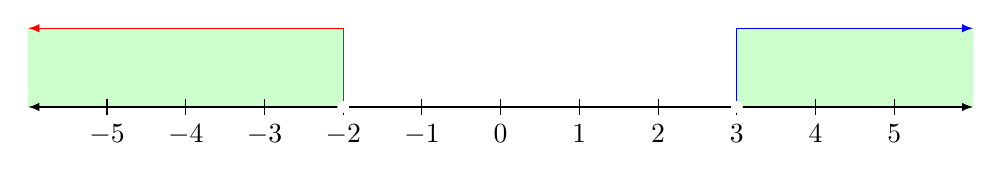
\begin{tikzpicture}
        \fill[green!20](-2,0)rectangle(-6,1);
        \fill[green!20](3,0)rectangle(6,1);
        \draw[latex-latex] (-6,0) -- (6,0) ;
        \foreach \x in {-5,-4,-3,-2,-1,0,1,2,3,4,5} \draw[shift={(\x,0)},color=black] (0pt,3pt) -- (0pt,-3pt) node[below] {$\x$};
        \node[circle,fill=white,inner sep=1.5pt](a)at(-2,0){};
        \node[circle,fill=white,inner sep=1.5pt](b)at(3,0){};
        %\node[circle,fill=black,inner sep=1.5pt](c)at(-3,0){};
        \draw[-latex,red](a)--++(0,1)--++(-4,0);
        \draw[-latex,blue](b)--++(0,1)--++(3,0);
    \end{tikzpicture}
    \caption{\color{blue}{Graphical representation of the domain of $y=\log\left(\dfrac{x-3}{x+2}\right)$}}
    \end{figure}

\newpage
    \begin{figure}[htbp]
        \centering
        \includegraphics[width=0.6\textwidth]{log1_17}
        \caption{\color{blue}{Graph of the function $y=\log\left(\dfrac{x-3}{x+2}\right)$ showing the domain $x\in (-\infty,-2)\cup(3,\infty)$. We also have two asymptotes at $x=-2$ and $x=3$}}
        %\label{fig:myimage}
    \end{figure}

\vspace{1in}
\begin{tcolorbox}[title=Domain and Asymptotes, colback=blue!10!white, colframe=blue!75!black]
Domain: Interval notation: $x\in (-\infty,-2)\cup(3,\infty)$\\
Domain: Set-builder notation: $\{ x \in \mathbb{R} \mid x<-2 \text{ and } x>3\}$\\
Asymptotes: $x=-2$ and $x=3$. 
\end{tcolorbox}

}



\newpage
\item $y=\ln\left(\sqrt{x-2}-1\right)$
{\color{blue}

The argument of the log should be strictly positive.  But the argument $x^2+1$ is always positive (this is a parabola $x^2$ that is shifted up 1 unit so it does not touch or cross the $x-$axis). So, there are no restrictions on $x$. The second term, $-3x$,  is a monomial and its domain is $\mathbb{R}$. 

Thus the domain of the function is $\mathbb{R}$ and it has no vertical asymptotes. This can be verified for the graph below. 

    \begin{align*}
        x+4>0 &\quad\text{and}\quad 2-x>0\\
        x> -4 &\quad\text{and}\quad x < 2
    \end{align*}

Put these results in a table to get region 

 \begin{figure}[!h]
    \centering    
\begin{tikzpicture}
\tkzTabInit[lgt=4,espcl=2,deltacl=0]
  { /.8, $x-2$ /.8, $\sqrt{x-2}-1$ /.8, overlap /.8}
  {,$2$,$3$,} % four main references
\tkzTabLine {,$\nexists$,z,+,t,+,} % seven denotations
\tkzTabLine {,$\nexists$,t,$\nexists$,z,+,}
\tkzTabLine {,$\nexists$,t,$\nexists$,t,+,}
\end{tikzpicture}
\caption{The tables shows the domain of the function is $x>3$}
\end{figure}



\vspace{1in}
The domain can also be represented graphically as shown below:
\vspace{0.5in}
\begin{figure}[!h]
    \centering
    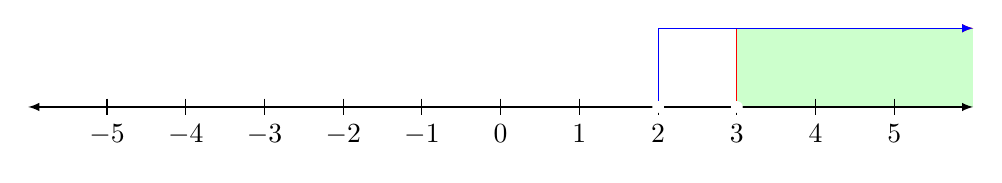
\begin{tikzpicture}
        \fill[green!20](6,0)rectangle(3,1);

        \draw[latex-latex] (-6,0) -- (6,0) ;
        \foreach \x in {-5,-4,-3,-2,-1,0,1,2,3,4,5} \draw[shift={(\x,0)},color=black] (0pt,3pt) -- (0pt,-3pt) node[below] {$\x$};
        \node[circle,fill=white,inner sep=1.5pt](a)at(3,0){};
        \node[circle,fill=white,inner sep=1.5pt](b)at(2,0){};
        %\node[circle,fill=black,inner sep=1.5pt](c)at(-3,0){};
        \draw[-latex,red](a)--++(0,1)--++(3,0);
        \draw[-latex,blue](b)--++(0,1)--++(4,0);
    \end{tikzpicture}
    \caption{\color{blue}{Graphical representation of the domain of $y=\ln\left(\dfrac{2-x}{\sqrt{x+4}}\right)$}}
    \end{figure}

\newpage
    \begin{figure}[htbp]
        \centering
        \includegraphics[width=0.6\textwidth]{log1_18}
        \caption{\color{blue}{Graph of the function $y=\ln\left(\sqrt{x-2}-1\right)$ showing the domain $x\in (3,\infty)$. We also have an asymptote at $x=3$}}
        %\label{fig:myimage}
    \end{figure}

\vspace{1in}
\begin{tcolorbox}[title=Domain and Asymptotes, colback=blue!10!white, colframe=blue!75!black]
Domain: Interval Notation: $x\in (3,\infty)$\\
Domain: Set-builder notation: $\{ x \in \mathbb{R} \mid x>3\}$\\
Asymptotes: $x=3$. 
\end{tcolorbox}
}

\end{enumerate}
